\documentclass[master]{finthesis}

\usepackage[pdftex]{graphicx}
\usepackage{amsmath}

\usepackage{caption}
\usepackage{subcaption}
\captionsetup[figure]{font=footnotesize, justification=centering}
%\captionsetup[table]{font=footnotesize}
\usepackage{tikz}
\usepackage{circuitikz}
%\usetikzlibrary{through, patterns}

%\usepackage[T1]{fontenc}

\usepackage[dvipsnames]{xcolor} % for more colors
\usepackage{amssymb} % for arrow symbol
\usepackage{tikz, pgfplots} % for diagram
\usepackage{schemabloc}  % for tikz trapezium
\usepackage{booktabs} % for bold lines in table
\usepackage{fancyhdr} % for header and footer

% For group PGF plots
\pgfplotsset{compat=newest}
\usetikzlibrary{pgfplots.groupplots}
\usepgfmodule{oo}

% Color variables
\def \CtrlColor        {darkgray}
\def \BBctrlColor      {RoyalBlue}
\def \PIDctrlColor     {OliveGreen}
\def \DCOColor         {BrickRed}
\def \CtrlDecColor     {brown}
\def \CtrlPreprocColor {RoyalPurple}
\def \ClkDivColor      {Goldenrod}
\def \RstnColor        {BurntOrange}

% Abbreviation variables
\def \PLL  {PLL} % phase-locked loop
\def \FLL  {FLL} % frequency-locked loop
\def \DLL  {DLL} % delay-locked loop
\def \DCO  {DCO} % digitally controlled oscillator 
\def \PID  {PID} % proportional-integral-derivative
\def \P    {P}   % proportional
\def \I    {I}   % integral
\def \D    {D}   % derivative
\def \FCW  {FCW} % frequency control word
\def \PWT  {PVT} % process-voltage-temperature
\def \HLLS {HLLS} % high-low level shifter
\def \LHLS {LHLS} % low-high level shifter


\addbibresource{master_rad.bib}

\title{Синтетизабилна дигитална фреквенцијски затворена петља са широким подешавањем до 640\texorpdfstring{\,}{ }MHz у 130\texorpdfstring{\,}{ }nm CMOS технологији}
\author{Ђорђе С. Гачић}
\studid{408/2022}
\advisor{проф. др Владимир М. Миловановић}
\advisorfull{Др Владимир М. Миловановић,\\ванредни професор}

\studprog{Електротехника и рачунарство}
% \module{Модул}
\course{Напредно машинско учење}
\date{\today}
% \date{ГГГГ-ММ-ДД}

\committee{др Шћепан Шћекић}
\committee{доц. др Жарко Попара}

\studentshould{% У оквиру овог рада кандидат треба да...
}

%\titlepagebib{greenwade93}
%\titlepagebib{pythonsite}
\titlepagebib{Staszewski:FREQUENCY_SYNTHESIZER_CMOS_2005}

\thesisapplicationfile{slike/prijava}

\abstracten{Frequency-locked loops (FLLs) represent a viable way of generating a range of frequencies from a single reference frequency by using a negative feedback electronic control system that compares the frequency of a controlled oscillator to the reference one. A digital synthesizable FLL is designed in 130\,nm CMOS technology for a target frequency of up to 640\,MHz. It employs a wide-tuning range digitally controlled oscillator (DCO) assembled from tri-state inverters in the form of a matrix. The FLL can optionally use a bang-bang or a soft-programmable standard proportional-integral-derivative (PID) controller to regulate the feedback loop. Its design practically minimizes metastability occurrence. The proposed digital FLL occupies 100\,\textmu m $\times$ 330\,\textmu m and consumes 3.5\,mW in typical operating conditions. The reference clock is 16\,MHz, and the output oscillation frequency is set to 640\,MHz, while the achieved frequency resolution is 2.8\,MHz.}
\keywordsen{Frequency-locked loop, digitally controlled oscillator, clock generator, synthesizable, CMOS technology, PID controller, metastability}

\abstractsr{Фреквенцијски затворене петље (енгл. \textsl{frequency-locked loops - FLLs}) представљају одржив начин генерисања опсега фреквенција из једне референтне фреквенције коришћењем електронског система управљања са негативном повратном спрегом, који пореди фреквенцију контролисаног осцилатора са поменутом референтном фреквенцијом. Дигитално синтетизабилан \FLL\ је дизајниран у 130\,nm технологији за циљану фреквенцију до 640\,MHz. Он погони дигитално контролисани осцилатор (енгл. \textsl{digitally-controlled oscillator - DCO}) са широким подешавањем опсега који се састоји од тростатаичких инвертора у облику матрице. \FLL\ може произвољно користити тзв. \textsl{bang-bang} контролер или дјелимично програмирани стандардни пропорционално-интегрално-диференцијални (енгл. \textsl{proportional-integral-derivative - PID}) контролер за управљање негативном петљом. Такав дизајн у пракси минимизује појаву метастабилности. Предложени дигитални \FLL\ заузима 100\,\textmu m $\times$ 330\,\textmu m простора и троши 3.5\,mW у уобичајеним условима рада. Референтни такт је 16\,MHz, а излазна фреквенција осциловања је подешена на 640\,MHz, док постигнута резолуција фреквенције износи 2.8\,MHz.}
\keywordssr{Фреквенцијски затворена петља, дигитално контролисани осцилатор, генератор такта, синтетизабилност, CMOS технологија, \PID\ контролер, метастабилност}

% Semantic markup. Look it up!
%\newcommand{\cmd}[2][]{\texttt{\textbackslash #2#1\{\ldots\}}} % Well, this one is useful beyond just semantics...
%\newcommand{\env}[1]{\texttt{#1}}
%\newcommand{\pkg}[1]{\texttt{#1}}
%\newcommand{\prog}[1]{\texttt{#1}}

\begin{document}

\maketitle

\tableofcontents

\makeabstract

\section{Увод}
У данашње вријеме, фазно затворена петља (енгл. \textsl{phase-locked loop - PLL)} и петља са затвореним кашњењем (енгл. \textsl{delay-locked loop - DLL}) представљају свеприсутне блокове у дизајну чипова. Безброј примјена самих чипова захтјевају или генератор такта или синтетизатор фреквенције, што подразумјева уградњу неког од поменутих блокова унутар система који се пројектује. Главна улога таквог блока у дизајну је да генерише стабилан и прецизан излазни сигнал чија је фаза подесива у односу на фазу улазног сигнала, самим тим одржавајући везу између улазне и излазне фреквенције. Међутим, чак и веома сложени системи често захтјевају генератор такта, који само множи улазну фреквенцију без да посебно води рачуна о фази такта или апсолутном подрхтавању (енгл. \textsl{jitter}). У таквим примјенама, потребна и довољна је само фреквенцијски затворена петља (енгл. \textsl{frequency-locked loop - FLL}) да би се испунили тражени захтјеви.

По дефиницији, \FLL\ је управљачки систем са негативном повратном спрегом који закључава фреквенцију излазног сигнала на предвиђену циљану фреквенцију. У принципу, непрастано управља фреквенцијом осцилатора на аутоматски начин све док излазна фреквенција на достигне циљану вриједност, након чега се та вриједност фреквенција одржава на излазу. Постоје многи начини имплементације \FLL-а~\cite{Ali:9097205}. Штавише, \FLL\ као интегрисано коло може спадати у двије групе: дигитални и аналогни \FLL. Иако је очигледан недостатак првих максимална фреквенција и њена резолуција, они посједују многе друге предности наспрам њихових аналогних супарника. Они заузимају мање простора, истичу се већом отпорношћу на промјене процесних углова, напона и температуре (енгл. \textsl{process-voltage-temperature - PVT}), лако су употребљиви у различитим технологијама, и стога омогућавају поновну употребу, већу прилагодљивост, једноставнију методологију тока пројектовања, као и брже циклусе пројектовања. Узимајући у обзир све претходно поменуто, испоставља се да је у општем случају боље ићи ка развоју дигиталног \FLL-a кад год спецификација архитектуре система то дозвољава. Дакле, фокус овог рада је пројектовати и унаприједити једноставне али моћне синтетизабилне дигиталне блокове чипа.

Овај рад конкретно предлаже синтетизабилан дигитални \FLL\ сличан предложеном у литератури~\cite{Musa:6644316}, са побољшаном брзином закључавања \FLL-а~\cite{Deng:6891375} и смањеним ризиком од метастабилности. Осцилатор је састављен од тростатичких инвертора и заснован на прстенастом \DCO-у из литературе~\cite{Tierno:4443210} измјењен додавањем независног напона напајања \DCO-а са претварачима напонских нивоа (енгл. \textsl{level shifters}) и употребом петостепене~\cite{Rylyakov:4523284} умјесто тростепене толологије прстена осцилатора.

Остатак рада укључује додатна поглавља. Поглавље \ref{FLL structure} описује предложени дигитални \FLL\ на системском нивоу и нивоу блокова и кола уз детаљна теоријска разматрања. Поглавље \ref{Implementation and results} пружа увид у имплементацију и добијене резултате симулација, такође уз теоријска разматрања појава које су од значаја за рад читавог система. Коначно, поглавље \ref{Conclusion} закључује рад и наговјештава могућности даљег рада на побољшању и проширењу система.


\section{Структура фреквенцијски затворене петље} \label{FLL structure}


У овом раду описана је релативно једноставна али ефикасна дигитална фреквенцијски затворена петља (\FLL). чију се системску архитектуру на нивоу блокова приказује \figurename~\ref{FLL block diagram}. Описани \FLL\ се практично састоји из два блока: дигитално контролисаног осцилатора (\DCO) и блока управљачке логике, који генерише улазне сигнале за \DCO\ на основу тренутне фреквенције \DCO-a. У сврху поједностављења, са слике су изостављени неки конфигурациони улази \FLL-a, као што су умножак фреквенције (енгл. \textsl{frequency control word - FCW}), коефицијенти \PID\ контролера и улаз за одабир режима рада. 

% FLL block diagram
\begin{figure*}[ht]
	\centering
	\begin{tikzpicture}[thick, scale=0.53, every node/.style={scale=0.45}]
		% Grid
		%\draw[step=1cm, gray, very thin] (0,0) grid (40,10);
		% Setup
		%\tikzset{every node/.style={align=center}};
		%\tikzstyle{every node}=[draw]
		% Beginning
		\draw                         (0  ,0) -- (0  ,5);
		\draw [-]                     (0  ,5) -- (1  ,5);
		\draw [-,  \CtrlColor]        (1  ,5) -- (1.5,5);
		\draw [->, \CtrlPreprocColor] (1.5,5) -- (1.94  ,5);
		% Preprocessing stage (grey counter + gra2bin conversion + synchronization)
		\node (GREYCNT)  at (2.8,5) [draw, \CtrlPreprocColor, minimum size=2cm, minimum height=2.4cm, align=center]{ГРЕЈЕВ  \\ БРОЈАЧ \\[5pt] \framebox{1,3,2,6}};
		\node (CONVSYNC) at (5.8,5) [draw, \CtrlPreprocColor, minimum size=2cm, minimum height=2.4cm, align=center]{СИНХР. \\ БИНАРНИ \\ ПРЕТВАРАЧ \\[5pt] \framebox{$\rightleftarrows$}};
		\draw [->, \CtrlPreprocColor] (GREYCNT) -- (CONVSYNC);
		\draw [dashed, \CtrlPreprocColor, fill=\CtrlPreprocColor, fill opacity=0.1, text opacity=1] (1.5,3.5) rectangle (7.5,6.5) node[midway, above=0.85]{УПРАВЉАЧКА ПРЕДОБРАДА};
		% Splitter/demultiplexer
		\node (DEMUX) at (8.5,5) [draw, \CtrlColor, trapezium, trapezium stretches=true, minimum width=7cm, minimum height=1cm, rotate=90]{ДЕМУЛТИПЛЕКСЕР};
		\draw [-,  \CtrlPreprocColor] (CONVSYNC) -- (7.5,5);
		\draw [->, \CtrlColor]           (7.5,5) -- (DEMUX);
		% Bang-bang FLL control branch
		\draw [-,    \CtrlColor]  (9  ,6.5) -- ( 9.5,6.5);
		\draw [->, \BBctrlColor] ( 9.5,6.5) -- (10  ,6.5);
		\node (CMP) at (11.4,6.5) [draw, \BBctrlColor, minimum size=2cm, minimum height=2.4cm, align=center]{КОМПАРАТОР \\[5pt] \framebox{$\geq$}};
		\node (CNT) at (14.2,6.5) [draw, \BBctrlColor, minimum size=2cm, minimum height=2.4cm, align=center]{БРОЈАЧ \\[5pt] \framebox{1,2,3}};
		\draw [->, \BBctrlColor]      (CMP) --      (CNT);
		\draw [-,  \BBctrlColor]      (CNT) -- (15.5,6.5);
		\draw [->,   \CtrlColor] (15.5,6.5) -- (16  ,6.5);
		\draw [dashed, \BBctrlColor, fill=\BBctrlColor, fill opacity=0.1, text opacity=1] (9.5,5) rectangle (15.5,8) node[midway, above=0.85]{ДВОСТЕПЕНИ РЕГУЛАТОР};
		% PID FLL control branch
		\draw [->, \CtrlColor] ( 9,3.5) -- (11,3.5);
		\node (PID) at (12.5,3.5) [draw, \PIDctrlColor, fill=\PIDctrlColor, fill opacity=0.1, text opacity=1, minimum width=3.5cm, minimum height=2.4cm, align=center]{\PID\ \\ РЕГУЛАТОР \\[5pt]};
		\draw [\PIDctrlColor] plot[smooth] coordinates {(11.75,2.7) (12.0,3.2) (12.5,3.1) (13.25,3.1)};
		\draw [\PIDctrlColor, fill=\PIDctrlColor, fill opacity=0.1] (11,2.5) rectangle (14,4.5) node[midway, below=0.6, opacity=1] {};
		\draw [->, \CtrlColor] (14,3.5) -- (16,3.5);
		% Control logic box
		\draw [dashed, \CtrlColor, fill=\CtrlColor, fill opacity=0.1, text opacity=1] (1,1) rectangle (21,9) node[midway, above=2.15]{УПРАВЉАЧКА ЛОГИКА};
		% Multiplexer
		\node (MUX) at (16.5,5) [draw, \CtrlColor, trapezium, trapezium stretches=true, minimum width=7cm, minimum height=1cm, rotate=-90]{МУЛТИПЛЕКСЕР};
		% Control Decoder
		\node (CTRLDEC) at (19,5) [draw, \CtrlDecColor, fill=\CtrlDecColor, fill opacity=0.1, text opacity=1, minimum size=2cm, minimum height=2.4cm, align=center]{УПРАВЉАЧКИ \\ ДЕКОДЕР};
		\draw [->, \CtrlColor] (MUX)  -- (CTRLDEC);
		% DCO
		\node (DCO) at (23,5) [draw, \DCOColor, fill=\DCOColor, fill opacity=0.1, text opacity=1, minimum size=2.4cm, minimum height=2.4cm, align=center]{DCO \\[5pt]};
		\draw [\DCOColor](22.8,4.7) sin (22.9,4.8) cos (23.0,4.7) sin (23.1,4.6) cos (23.2,4.7);
		\draw [\DCOColor](23.0,4.7) circle (0.3);
		\draw [-, \CtrlColor] (CTRLDEC) -- (21,5);
		\draw [->]                     (21,5) --  (DCO);
		% End
		\draw  (DCO) -- (25,5);
		\draw (25,5) -- (25,0);
		\draw (25,0) --  (0,0);
		
        \draw (-1,-1) rectangle (26,10) node[midway, above=2.95]{\textbf{ДИГИТАЛНА ФРЕКВЕНЦИЈСКИ ЗАТВОРЕНА ПЕТЉА}};	
        \draw [thick, ->] (-2.5,9) -- (-1,9) node[midway, above=0.1] {\textbf{RSTN}};
        \draw [thick, ->] (-2.5,8) -- (-1,8) node[midway, above=0.1] {\textbf{FREF}};        	
        \draw [thick, ->] (-2.5,7) -- (-1,7) node[midway, above=0.1] {\textbf{FMUL}};
        \draw [thick, ->] (-2.5,6) -- (-1,6) node[midway, above=0.1] {\textbf{CTRL}};
        \draw (-2.0,6.825) --  (-1.5,7.175);
        \draw (-2.0,5.825) --  (-1.5,6.175);
        %\draw [-]  (25,5) -- (26,5);
        \draw [thick, ->] (26,8) -- (27.5,8) node[midway, above=0.1] {\textbf{FOUT}};
        \draw [thick, ->] (26,7) -- (27.5,7) node[midway, above=0.1] {\textbf{LOCK}};
        
		
	\end{tikzpicture}
	\caption{Блок дијаграм дигиталне фреквенцијски затворене петље састављене од: блока управљачке логике (лијево) и дигитално контролисаног осцилатора (десно).}
	\label{FLL block diagram}
\end{figure*}


\subsection{Управљачка логика дигиталне фреквенцијски затворене петље}
Управљачка логика \FLL-a састоји се од двије независне процесне гране, које представљају два међусобно искључива режима управљања \FLL-a. Оба режима на улазу примају бинарну вриједност повезану са бројем периода такта \DCO-а унутар периода референтног такта. Такође, оба управљачка режима генеришу бинарну вриједност на излазу, која представља управљачку бинарну ријеч осцилатора директно пропорционалну излазној фреквенцији. Главне разлике између два поменута режима су брзина затварања (закључавања) \FLL-a и једноставност подешавања. Циљ управљачке логике \FLL-a је изједначити вриједност улазног множача фреквенције са бројем периода такта \DCO-a унутар периода референтног такта што је брже и прецизније могуће одрадити, чиме се долази до постизања жељене фреквенције на излазу \DCO-a. Комплетна управљачка логика \FLL-a је подјељена на неколико фаза, које су описане у наредним поглављима.

\subsubsection{Управљачка предобрада}
Фаза управљачке предобраде (енгл. \textsl{control preprocessing}) укључује неколико блокова чија је функција претворити информацију о фреквенцији излазног такта \DCO-a у бинарну вриједност која ће бити прослијеђена као улаз наредној фази управљачке логике \FLL-a. Као прво, да би се одредила брзина осциловања \DCO-a, потребан је бројач. У имплементацији описаној у овом раду коришћен је Грејев бројач умјесто природног бинарног бројача из разлога што значајно умањује метастабилност бројача изазвану узорковањем (енгл. \textsl{sampling}), јер у Грејевом коду свака узастопна вриједност се разликује за по један бит. Недостатак овог приступа је то што Грејев бројач има мању максималну радну фреквенцију од бинарног бројача. Да би се у још већем обиму смањио ризик од метастабилности, сваки бит са излаза Грејевог бројача се пропушта кроз синхронизатор са два флип-флопа да би безбједно прешао у подручје референтног такта. Затим, синхронизована вриједност Грејевог бројача се претвара у бинарни формат и узоркује се за даљу обраду.
% TODO
% Нешто више о Грејевом бројачу

\subsubsection{Bang-bang контролер}
Први управљачки блок \FLL-a је веома сличан bang-bang (или on-off) контролеру, односно контролеру са повратном спрегом који, као прекидач, може имати два стања. Он пореди улазни умножак фреквенције са узоркованом вриједношћу бројача и одлучује да ли инкрементирати, декрементирати или онемогућити предстојећи блок тј. двосмјерни бројач (енгл. \textsl{up-down counter}). То осигурава постепено управљање и закључавање све до постизања жељене фреквенције.

% TODO
% Нешто више о bang-bang контролеру

\subsubsection{\PID~контролер}
У другом управљачком режиму, управљачка бинарна ријеч за \DCO\ се генерише подесивим \PID\ контролером. \PID\ контролер је управљачки механизам заснован на повратној спрези, који ради тако што непрекидно исправља и скалира сигнал грешке, који је разлика између измјерене вриједности у обради (узоркована вриједност бројача) и жељене референтне задате вриједности (вриједност улазног умношка фреквенције). Исправљање и скалирање се распоређује у три компоненте: пропорционална (\P), интегрална (\I) и диференцијална (\D), имплементиране као подесиви улази са фиксном тачком који се напајају из банке регистара. \par
Сврха \P\ компоненте је да управља брзином одзива управљачког система, непосредно множећи сигнал грешке константним чиниоцем. \I\ компонента се користи за смањење грешке стабилног стања (енгл. \textsl{steady-state}) скалирањем грешке константним чиниоцем и сумирањем резултата током времена. \D\ компонента пропорционална брзини промјене грешке, и њен циљ је ограничити излаз да би се смањила могућа прекорачења или осцилације узроковане \P\ и \I\ компонентама, без смањења брзине контролера. Како је у овом систему референтна задата вриједност константна и нема брзих промјена на улазу које могу изазвати такав исход, \P\ и \I\ компоненте су довољне за гладак и стабилан одзив система.  

% TODO
% Нешто више о PID контролеру

\subsubsection{Управљачки декодер} \label{control decoder}
Улога управљачког декодера је претворити управљачке податке из једне бинарне вриједности у скуп управљачких улаза \DCO-а. Постоје три таква улаза: \textsl{Row On}, унарни вектор, који може да укључује читаве редове тростатичких инвертора \DCO-a; \textsl{Row Select}, један од $n$ вектор (енгл. \textsl{one-hot vector}), који укључује један додатни ред тростатичких инвертора \DCO-a; и \textsl{Column Select}, унарни вектор, који може да укључује колоне тростатичких инвертора \DCO-a. Да би се један инвертор укључио, или \textsl{Row On}, или и \textsl{Row Select} и \textsl{Column Select} за одговарајући бит морају бити подешени на 1. Ширина сваког вектора је једнака ширини улаза. Сама структура \DCO-a је детаљније описана у поглављу \ref{DCO structure}.

% TODO
% Нешто више о унарном и један од n кодирању

\subsection{Структура дигитално контролисаног осцилатора} \label{DCO structure}
У срцу сваке фазно затворене петље се налази осцилатор који игра кључну улогу у учинку који може бити постигнут~\cite{Razavi:PLL_CMOS_2020}. Дигитално контролисани осцилатор описан у овом раду је прстенасти осцилатор, погодан за систем генерисања такта. Прстенасти осцилатор је каскадна комбинација фаза кашњења повезаних у ланац затворене петље~\cite{Madhusudhana:283751064}. Прстенасте архитектуре су компактније од LC осцилатора и имају доста предности захваљујући својој правилној и периодичној просторној структури. Уопштена структура \DCO-а коришћеног унутар описаног \FLL-а заснована је на матрици тростатичких CMOS инвертора~\cite{Terosiet:340277809}. Ова матрица је састављена од $N$-фазних прстена тростатичких инвертора повезаних паралелно. $N$ представља број \DCO\ фаза (степени) и мора бити непаран број већи или једнак 3.
%(за осцилатор са једним излазним сигналом у односу на заједничко уземљење)
У физичком смислу, матрица може бити преобликована у квадрат, што омогућава једноставнију управљачку логику. Један или више прстенова су увијек укључени и дефинишу основну фреквенцију \DCO-а. Остали тростатички инвертори се укључују и искључују у зависности од управљачке логике. \par
Формула за фреквенцију осциловања конкретне имплементације \DCO-а из овог рада гласи:
\begin{equation} \label{f_osc}
    f_\text{osc} = \dfrac{1}{2Nt_\text{d}} \approx \dfrac{I_\text{d}}{2NC_\text{load}V_\text{DDL}}
\end{equation}
гдје је $N$ број тростатичких инвертора унутар прстена, $t_\text{d}$ представља кашњење једне ћелије \DCO-a, у чијем саставу је тростатички инвертор (у наставку ће бити детаљније објашњена структура саме ћелије \DCO-а), $I_\text{d}$ је струја која протиче кроз инвертор, $C_\text{load}$ је капацитивно оптерећење истог инвертора, и $V_\text{DDL}$ је напон напајања \DCO-а. Производ $Nt_\text{d}$ је помножен са $2$ да би се добила читава периода такта, а не полупериода.

\subsubsection{Предложена архитектура DCO-a}
Када је рijеч о топологији, са повећањем броја \DCO\ фаза (степени), фреквенцијски корак ($K_\text{DCO}$) опада, чиме се повећава прецизност \DCO-а. Максимална фреквенција осцилатора се се такође смањује, и да би се то надомјестило, напон напајања се може повећати, што с друге стране доводи до веће потрошње снаге. Ако претпоставимо да напон напајања и капацитивно оптерећење по једној фази остану непромјењени, повећање броја фаза не утиче на потрошњу снаге. Међутим, ако укупан број тростатичких инвертора остане непромјењен и подијели се на већи број фаза, то ће довести до смањења капацитивног оптерећења по фазама појединачно, што даље доводи до смањења потрошње снаге. Математичком анализом се то може објаснити на следећи начин: $N$-фазни прстенасти осцилатор који ради на фреквенцији $f_\text{osc}$ има динамичку потрошњу снаге која се може представити једначином
\begin{equation} \label{dynamic power}
    	P = N f_\text{osc} C_\text{tot} V^{2}_\text{DDL}, 
\end{equation}
гдје $C_\text{tot}$ представља укупно капацитивно оптерећење на једној фази. Пошто је фреквенција осциловања једнака
\begin{equation}
	f_\text{osc} = \frac{1}{2Nt_\text{d}},
\end{equation}
једначину за динамичку снагу можемо написати на следећи начин:
\begin{equation}
    	P = \frac{C_\text{tot}V^{2}_\text{DDL}}{2t_\text{d}},
\end{equation}
одакле се види да је добијена динамичка снага независна од $N$~\cite{Razavi:PLL_CMOS_2020}. \par

У овом раду описана је топологија \DCO-a са пет фаза, због тога што је таквом топологијом остварен задовољавајући компромис између учинка и потрошње снаге. \figurename~\ref{DCO5} приказује структуру \DCO-а коришћеног у описаној \FLL\ имплементацији. 
\pgfooclass{InvRow}{
    \method InvRow(){}
    \method apply(#1,#2,#3){
        \draw 
        (#1,#2) node[ieeestd not port, anchor=in, scale=0.4, fill=ColorPhase0, fill opacity=\InvFillOpacity]({#3}0){}
        ({#3}0.out) node[ieeestd not port, anchor=in, scale=0.4, fill=ColorPhase1, fill opacity=\InvFillOpacity]({#3}1){}
        ({#3}1.out) node[ieeestd not port, anchor=in, scale=0.4, fill=ColorPhase2, fill opacity=\InvFillOpacity]({#3}2){}
        ({#3}2.out) node[ieeestd not port, anchor=in, scale=0.4, fill=ColorPhase3, fill opacity=\InvFillOpacity]({#3}3){}
        ({#3}3.out) node[ieeestd not port, anchor=in, scale=0.4, fill=ColorPhase4, fill opacity=\InvFillOpacity]({#3}4){};
    }
}
\begin{figure*}[!ht]
\centering
\begin{tikzpicture}[scale=0.95]
    \ctikzset{tripoles/mos style/arrows}
    \ctikzset{tripoles/pmos style/emptycircle}
    \ctikzset{logic ports=ieee}

    \definecolor{ColorPhase0}{RGB}{255,0,0}
    \definecolor{ColorPhase1}{RGB}{192,0,64}
    \definecolor{ColorPhase2}{RGB}{128,0,128}
    \definecolor{ColorPhase3}{RGB}{64,0,192}
    \definecolor{ColorPhase4}{RGB}{0,0,255}

    \definecolor{HLLSColor}{RGB}{64,0,77}
    \definecolor{LHLSColor}{RGB}{106,0,128}

    \definecolor{AlwaysOnBoxColor}{RGB}{0,255,0}
    
    % Color opacity variables
    \def \InvFillOpacity      {1}
    \def \DCOFillOpacity      {0.05}
    \def \CtrlDecFillOpacity  {0.1}
    \def \AlwaysOnBoxOpacity  {0.1}
    \def \HLLSFillOpacity     {0.1}
    \def \HLLSTextOpacity     {1}
    \def \LHLSFillOpacity     {0.05}
    \def \LHLSTextOpacity     {1}
    %
    \pgfoonew \invRow=new InvRow()
    %
    % LEFT INVERTER MATRIX
    \invRow.apply(0,0,i0)
    \invRow.apply(0,0.8,i1)
    \invRow.apply(0,1.6,i2)
    %
    \foreach \x in {0,1,2,3,4}
        \draw ({i0}\x.out) -- ({i1}\x.out) -- ({i2}\x.out) --++ (0,0.5) node[anchor=west, rotate=90, scale=0.5](lcont\x){...};
    \draw ({i0}0.in) -- ({i1}0.in) -- ({i2}0.in) --++ (0,0.5) node[anchor=west, rotate=90, scale=0.5](lcont5){...};
    %
    \invRow.apply(0,3,i3)
    \invRow.apply(0,3.8,i4)
    \invRow.apply(0,4.6,i5)
    %
    \foreach \x in {0,1,2,3,4}
        \draw (lcont\x.east) -- ({i3}\x.out) -- ({i4}\x.out) -- ({i5}\x.out);
    \draw (lcont5.east) -- ({i3}0.in) -- ({i4}0.in) -- ({i5}0.in);
    %
    % RIGHT INVERTER MATRIX
    \invRow.apply(5.8,0,ii0)
    \invRow.apply(5.8,0.8,ii1)
    \invRow.apply(5.8,1.6,ii2)
    %
    \foreach \x in {0,1,2,3,4}
        \draw ({ii0}\x.out) -- ({ii1}\x.out) -- ({ii2}\x.out) --++ (0,0.5) node[anchor=west, rotate=90, scale=0.5](rcont\x){...};
    \draw ({ii0}0.in) -- ({ii1}0.in) -- ({ii2}0.in) --++ (0,0.5) node[anchor=west, rotate=90, scale=0.5](rcont5){...};
    %
    \invRow.apply(5.8,3,ii3)
    \invRow.apply(5.8,3.8,ii4)
    \invRow.apply(5.8,4.6,ii5)
    %
    \foreach \x in {0,1,2,3,4}
        \draw (rcont\x.east) -- ({ii3}\x.out) -- ({ii4}\x.out) -- ({ii5}\x.out);
    \draw (rcont5.east) -- ({ii3}0.in) -- ({ii4}0.in) -- ({ii5}0.in);
    %
    % RECTANGLE FOR ALWAYS ON INVERTERS
    \draw 
    ({i0}0.in) ++ (-0.2,-0.4) node[](ron1){}
    ({i0}0.in) ++ (-0.2,0.4) node[](ron2){}
    ({ii0}4.out) ++ (0.2,0.4) node[](ron3){}
    ({ii0}4.out) ++ (0.2,-0.4) node[](ron4){};
    \filldraw[draw, AlwaysOnBoxColor, fill=AlwaysOnBoxColor, fill opacity=\AlwaysOnBoxOpacity] (ron1.center) -- (ron2.center) -- (ron3.center) -- (ron4.center) -- (ron1.center);
    %
    % UPPER PHASE CONNECTIONS
    \draw ({i5}4.out) ++ (0,1.1) |-++ (0,0.2) node[circ, scale=0.4](circ1){} --++ (0.5,0) node[anchor=west, scale=0.5](contp0){...}
    (contp0.east) -| ({ii5}4.out);
    \draw [dashed] ({i5}4.out) --++ (0,1.1);
    \draw [dashed] ({ii5}0.in) --++ (0,1.1);
    \draw ({ii5}0.in) ++ (0,1.1) --++ (0,0.2) node[circ, scale=0.4](circ2){}
    ({i5}0.in) |- (circ1);
    \foreach \x/\y in {0/1, 1/2, 2/3, 3/4} {
        \draw 
        (contp\x.west) ++ (0,-0.2) node[anchor=west, scale=0.5](contp\y){...}
        ({i5}\x.out) |- (contp\y.west)
        (contp\y.east) -| ({ii5}\x.out);
    }
    \draw
    ({i4}4.out) ++ (0.5,0) node[anchor=west, scale=0.5](contc0){...}
    ({i1}4.out) ++ (0.5,0) node[anchor=west, scale=0.5](contc1){...};
    %
    % BOTTOM ARROWS FOR ALL INVERTERS
    \foreach \r in {0,1,2,3,4,5}{
        \foreach \c in {0,1,2,3,4}{
            \draw ({i\r}\c.down) node[inputarrow, rotate=90, scale = 0.8]{} --++ (0,-0.3);
            \draw ({ii\r}\c.down) node[inputarrow, rotate=90, scale = 0.8]{} --++ (0,-0.3);
        };
    };
    %
    % DCO RECTANGLE
    \draw
    ({i0}0.in) ++ (-0.5,-1.2) node[](r1){}
    ({i5}0.in) ++ (-0.5,1.6) node[](r2){}
    ({ii5}4.out) ++ (0.5,1.6) node[](r3){}
    ({ii0}4.out) ++ (0.5,-1.2) node[](r4){}
    (r1) node[anchor=south west](){DCO};
    \filldraw[draw, \DCOColor, fill=\DCOColor, fill opacity=\DCOFillOpacity] (r1.center) -- (r2.center) -- (r3.center) -- (r4.center) -- (r1.center);
    %
    % COLUMN CONTROL RECTANGLE
    \draw
    (r2) ++ (0.5,1.8) node[](rc1){} 
    (r3) ++ (-0.5,1.8) node[](rc4){}
    (rc1) ++ (0,0.5) node[](rc2){}
    (rc4) ++ (0,0.5) node[](rc3){}
    ($(rc1)!0.5!(rc4)$) node[anchor=south, scale=0.8, text=\CtrlDecColor]{Управљање колонама};
    \filldraw[draw, \CtrlDecColor, fill=\CtrlDecColor, fill opacity=\CtrlDecFillOpacity] (rc1.center) -- (rc2.center) -- (rc3.center) -- (rc4.center) -- (rc1.center);
    %
    % HLLS FROM COLUMN CONTROL RECTANGLE
    \foreach \i/\x in {0/0.4, 1/1.15, 2/1.9, 3/2.65, 4/3.4, 5/6.2, 6/6.95, 7/7.7, 8/8.45, 9/9.2} {
        \draw
        (rc1) ++ (\x,0) --++ (0,-0.4) node[inputarrow, rotate=-90](){} node[rectangle, minimum size=3, thick, rotate=-90, anchor=west, scale=0.7, color=HLLSColor, fill=HLLSColor, fill opacity=\HLLSFillOpacity, text opacity=\HLLSTextOpacity, draw](hl\i){HLLS}
        (hl\i.east) --++ (0,-0.4) node[inputarrow, rotate=-90](){};
    }
    \draw
    (hl4.north) ++ (0.67,0) node[anchor=west, scale=0.5](){...}
    %
    % ROW CONTROL RECTANGLE
    (r1) ++ (-1.8,1.6) node[](rr1){} 
    (r2) ++ (-1.8,-1.2) node[](rr4){}
    (rr1) ++ (-0.5,0) node[](rr2){}
    (rr4) ++ (-0.5,0) node[](rr3){}
    ($(rr1)!0.5!(rr4)$) node[anchor=north, scale=0.8, rotate=-90, text=\CtrlDecColor]{Управљање редовима};
    \filldraw[draw, \CtrlDecColor, fill=\CtrlDecColor, fill opacity=\CtrlDecFillOpacity] (rr1.center) -- (rr2.center) -- (rr3.center) -- (rr4.center) -- (rr1.center);
    %
    % HLLS FROM ROW CONTROL RECTANGLE
    \foreach \i/\y in {0/0.4, 1/1.2, 2/2.5, 3/3.3, 4/4.1} {
        \draw
        (rr1) ++ (0,\y) --++ (0.4,0) node[inputarrow](){} node[rectangle, minimum size=3, thick, anchor=west, scale=0.7, color=HLLSColor, fill=HLLSColor, fill opacity=\HLLSFillOpacity, text opacity=\HLLSTextOpacity, draw](hlr\i){HLLS}
        (hlr\i.east) --++ (0.4,0) node[inputarrow](){};
    }
    \draw 
    (hlr1.north) ++ (0,0.3) node[anchor=west, rotate=90, scale=0.5](){...}
    %
    % LHLS AND PHASE PORTS
    ($(r3)!0.5!(r4)$) node[](rph2){}
    (rph2) ++ (0,0.7) node[](rph1){}
    (rph1) ++ (0,0.7) node[](rph0){}
    (rph2) ++ (0,-0.7) node[](rph3){}
    (rph3) ++ (0,-0.7) node[](rph4){};
    %
    \foreach \i in {0,1,2,3,4} {
        \draw
        (rph\i.center) --++ (0.4,0) node[inputarrow](){} node[rectangle, minimum size=3, thick, anchor=west, scale=0.7, color=LHLSColor, fill=LHLSColor, fill opacity=\LHLSFillOpacity, text opacity=\LHLSTextOpacity, draw](lh\i){LHLS} 
        (lh\i.east) --++ (0.4,0) node[signal, anchor=west, fill=ColorPhase\i, draw](ph\i){} node[inputarrow](){}
        (ph\i.east) node[anchor=west, scale=0.8]{Фаза \i};
    }
\end{tikzpicture}
\caption{Петостепени прстенасти дигитално контролисани осцилатор (\DCO) састављен од тростатичких инвертора, са додатим претварачима напонских нивоа (\HLLS\ и \LHLS) и уоквиреним редом стално укључених тростатичких инвертора.}
\label{DCO5}
\end{figure*}
 \par
Свака фаза \DCO-а састоји се од 54 тростатичка инвертора, што ако помножимо са бројем фаза даје укупно 270 инвертора. Тростатички инвертори су распоређени у 18 редова и 15 колона. Управљачка логика \FLL-a управља са 17 редова и свих 15 колона, што значи да постоји 255 фреквенцијских корака. Преостали ред са 3$\times$5 тростатичких инвертора је увијек укључен и на њега не утиче управљачка логика \FLL-а. Што се више тростатичких инвертора у свакој фази укључи под утицајем управљачке логике \FLL-а, тренутна снага покретања (енгл. \textsl{driving strength}) једне фазе се повећава, док њено капацитивно оптерећење у суштини остаје константно, што резултује повећањем излазне фреквенције осциловања~\cite{Tierno:4443210}.

\subsubsection{Блок дијаграм DCO ћелије}
Да би се ефикасно подесила излазна фреквенција \DCO-а, уведен је скуп управљачких улаза \DCO-а, а то су сигнали \textsl{Row On}, \textsl{Row Select} и \textsl{Column Select}, поменути такође у секцији \ref{control decoder}. Према томе, сваки тростатички инвертор појединачно садржи сопствену управљачку јединицу у облику И-ИЛИ стандардне ћелије, и заједно граде већи блок назван ћелија \DCO-а. \figurename~\ref{DCO_cell} приказује шему ћелије \DCO-а на нивоу логичких кола и на нивоу CMOS транзистора.
\begin{figure}[!ht]
    \centering
    %\vspace{0.7cm}
    \subfloat[]{
    \begin{tikzpicture}[scale=1]
        \ctikzset{tripoles/mos style/arrows}
        \ctikzset{tripoles/pmos style/emptycircle}
        \ctikzset{logic ports=ieee}
        \draw (0,0)
        node[ieeestd not port, anchor=out, scale=1](tsinv){}
        (tsinv.in) --++ (-0.5,0) node[signal, anchor=east, scale=1, draw](pinphi){} 
        (pinphi.west) node[anchor=east, scale=1]{In}
        %(tsinv.in) --++ (0,-1.3) --++ (-8.5,0) node[anchor=east, scale=1](inlong){In}
        %(inlong) --++ (-0.5,0) node[signal, anchor=east, scale=1, draw](pinphi){} 
        (tsinv.out) --++ (0.4,0) node[signal, anchor=west, scale=1, draw](pinpho){} 
        (pinpho.east) node[anchor=west, scale=1]{Out}
	(tsinv.up) --++ (0,0.4) node[anchor=west, scale=1]{ctrl} |-++ (-3.5,0.2) node[ieeestd not port, anchor=out, scale=1](not) {} 
	(tsinv.down) --++ (0,-0.4) node[anchor=west, scale=1]{$\overline{\mbox{ctrl}}$}
	(not.in) --++ (-1,0) node[ieeestd nor port, anchor=out, scale=1](nor){}
        (nor.in 2) -|++ (0, -0.6) node[ieeestd and port, anchor=out, scale=1](and){}
        (nor.in 1) -- (and.in 1|-nor.in 1) node[signal, anchor=east, scale=1, draw](pinro){} 
        (pinro.west) node[anchor=east, scale=1]{Row On}       
        (and.in 1) node[signal, anchor=east, scale=1, draw](pinrs){} 
        (pinrs.west) node[anchor=east, scale=1]{Row Sel.}
        (and.in 2) node[signal, anchor=east, scale=1, draw](pincs){} 
        (pincs.west) node[anchor=east, scale=1]{Col. Sel.};
	\draw[-] (not.in) node[circ]{} --++ (0,-1.8) -| (tsinv.down);
	\draw[dashed] (and.in 2) ++ (0.2,0) node[](csin){} --++ (0,2.5) -| (not.out) --++ (0,-2.9) -| (csin);
	\draw[dashed] (not.in) ++ (-0.3,0) node[](notin){} --++ (0,1) -| (tsinv.out) --++ (0,-1.7) -| (notin);
	\draw (csin) ++ (2.5,2.5) node[anchor=south west](andorlabel){\small И-ИЛИ}; 
	\draw (csin) ++ (7,2.1) node[anchor=south west](tsinvlabel){\small Тростатички инвертор}; 
	%\draw[dashed] (not.out) --++ (0,0.9);
	\draw[thick] (tsinv.down) node[draw, circle, anchor=north, fill=white, minimum size=0.17cm, inner sep=0] (invup) {};
        %\draw[decoration={brace, mirror},decorate] (not.out) ++ (0,0.9) --++ (-3.25,0) node[above=2pt] {\small И-ИЛИ} --++ (-3.23,0);
    \end{tikzpicture}
    %\vspace{0.2cm}
    \label{DCO_cell_logic_gate_level}
    }
    \vfil
    %\hfil
    \vspace{0.5cm}
    \subfloat[]{
    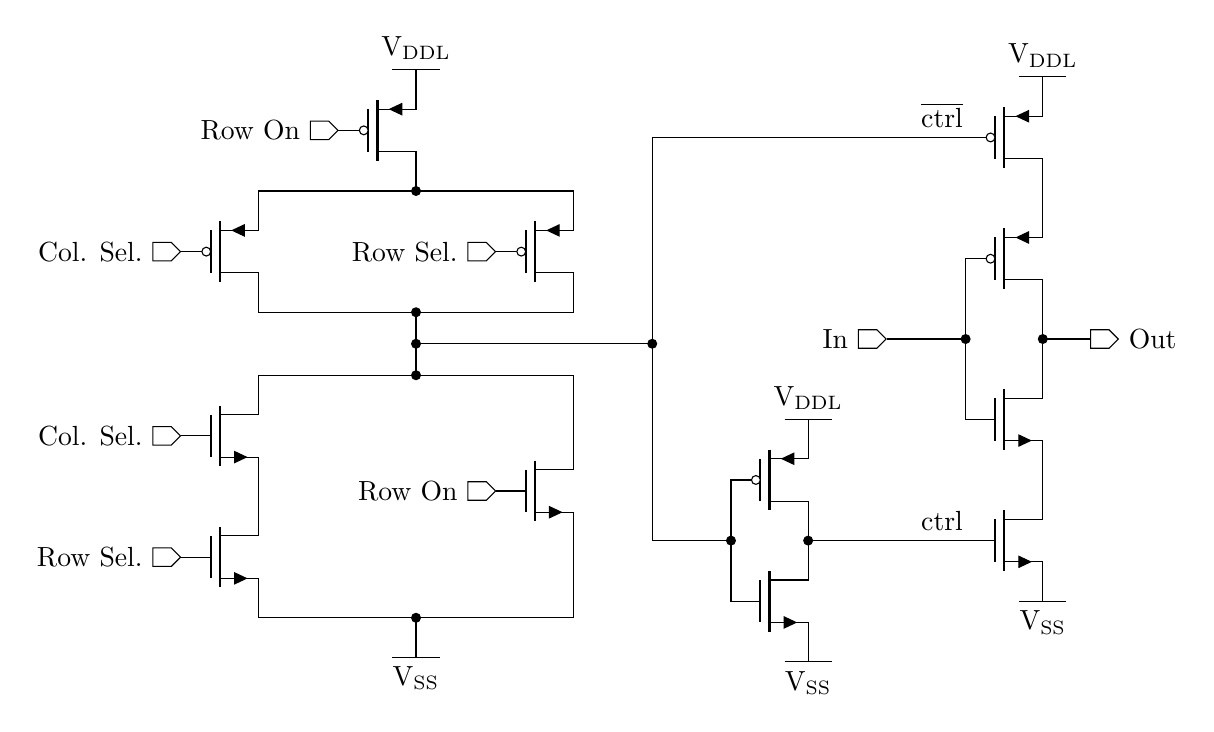
\begin{tikzpicture}[scale=1]
        \ctikzset{tripoles/mos style/arrows}
        \ctikzset{tripoles/pmos style/emptycircle}
        \ctikzset{logic ports=ieee}
        \draw (0,0)
        node[pmos, scale=1](pmos1){}
        (pmos1.D) to [short] ++(0,-0.5) node[nmos, scale=1, anchor=D](nmos1){}
        (pmos1.G) to (nmos1.G)
        ($(pmos1.G)!0.5!(nmos1.G)$) node[circ, scale=1]{} --++ (-1,0) node[signal, anchor=east, scale=1, draw](pinphi){} 
        (pinphi.west) node[anchor=east, scale=1]{In}
        ($(pmos1.D)!0.5!(nmos1.D)$) node[circ, scale=1]{} --++ (0.6,0) node[signal, anchor=west, scale=1, draw](pinpho){} 
        (pinpho.east) node[anchor=west, scale=1]{Out}
        (pmos1.S) node[pmos, scale=1, anchor=D](pmos2){}
        (pmos2.G) ++(-0.3,0) node[anchor=south, scale=1]{$\overline{\mbox{ctrl}}$}
        (nmos1.S) node[nmos, scale=1, anchor=D](nmos2){}
        (nmos2.G) --++ (-1,0) |-++ (-1,0) node[circ, scale=1](nctrl){}
        (nmos2.G) ++ (-0.3,0) node[anchor=south, scale=1]{ctrl}
        (nctrl) node[pmos, scale=1, anchor=D](pinv){}
        (nctrl) node[nmos, scale=1, anchor=D](ninv){}
        (pinv.G) to (ninv.G)
        ($(pinv.G)!0.5!(ninv.G)$) node[circ, scale=1]{} --++ (-1,0) --++ (0,2.5) node[circ, scale=1](pctrl){} |- (pmos2.G)
        (pctrl) --++ (-3,0) node[circ, scale=1](ctrl){}
        (ctrl) --++ (0,0.4) node[circ, scale=1](pside){}
        (ctrl) --++ (0,-0.4) node[circ, scale=1](nside){}
        (pside) ++ (2,0) node[pmos, scale=1, anchor=D](prs){}
        (pside) ++ (-2,0) node[pmos, scale=1, anchor=D](pcs){}
        (prs.G) node[signal, anchor=east, scale=1, draw](pinrs){} 
        (pinrs.west) node[anchor=east, scale=1]{Row Sel.}
        (pcs.G) node[signal, anchor=east, scale=1, draw](pincs){} 
        (pincs.west) node[anchor=east, scale=1]{Col. Sel.}
        (prs.D) to (pcs.D)
        (prs.S) to (pcs.S)
        ($(pcs.S)!0.5!(prs.S)$) node[circ, scale=1]{} node[pmos, scale=1, anchor=D](pro){}
        (pro.G) node[signal, anchor=east, scale=1, draw](pinro){} 
        (pinro.west) node[anchor=east, scale=1]{Row On}
        %
        (nside) ++ (-2,0) node[nmos, scale=1, anchor=D](ncs){}
        (nside) -|++ (2,-0.7) node[nmos, scale=1, anchor=D](nro){}
        (ncs.G) node[signal, anchor=east, scale=1, draw](pinncs){} 
        (pinncs.west) node[anchor=east, scale=1]{Col. Sel.}
        (nro.G) node[signal, anchor=east, scale=1, draw](pinnro){} 
        (pinnro.west) node[anchor=east, scale=1]{Row On}
        (ncs.D) to (nside)
        (ncs.S) node[nmos, scale=1, anchor=D](nrs){}
        (nrs.G) node[signal, anchor=east, scale=1, draw](pinnrs){} 
        (pinnrs.west) node[anchor=east, scale=1]{Row Sel.}
        (nrs.S) --++ (2,0) node[circ, scale=1](vss){} -| (nro.S)
        %
        (vss) --++ (0, -0.5) node[](vss1){} ++ (-0.3,0) --++ (0.6,0) 
	(vss1) node[anchor=north, scale=1]{$\text{V}_\text{SS}$}
        (ninv.S) ++ (-0.3,0) --++ (0.6,0)
	(ninv.S) node[anchor=north, scale=1]{$\text{V}_\text{SS}$}
        (nmos2.S) ++ (-0.3,0) --++ (0.6,0)
	(nmos2.S) node[anchor=north, scale=1]{$\text{V}_\text{SS}$}
        (pmos2.S) ++ (-0.3,0) --++ (0.6,0)
	(pmos2.S) node[anchor=south, scale=1]{$\text{V}_\text{DDL}$}
        (pro.S) ++ (-0.3,0) --++ (0.6,0)
	(pro.S) node[anchor=south, scale=1]{$\text{V}_\text{DDL}$}
        (pinv.S) ++ (-0.3,0) --++ (0.6,0)
	(pinv.S) node[anchor=south, scale=1]{$\text{V}_\text{DDL}$}
        ;
    \end{tikzpicture}
    \label{DCO_cell_transistor_level}
    }
    \caption{Ћелија \DCO-а на нивоу (a) логичких кола и (б) CMOS транзистора.}
    \label{DCO_cell}
\end{figure}


\subsubsection{Претварачи напонских нивоа DCO-a}
Напон напајања који користи дигитално контролисани осцилатор ($V_\text{DDL}$) се разликује од напона напајања који користи остатак логике \FLL-а ($V_\text{DD}$). Предност таквог дизајна је могућност подешавања напона напајања \DCO-а независно након производње чипа, што даље омогућава постизање жељене резолуције фреквенције (фреквенцијског корака) и фреквенцијског опсега зависно од процесног угла у коме се одвијала производња чипа. Додатна предност јесте и то што могућност смањења напона напајања \DCO-а аутоматски доводи и до значајног смањења расипања снаге (енгл. \textsl{power disipation}) због њене квадратне зависности од напона напајања.
Независан домен напајања \DCO-а постигнут је додавањем претварача напонских нивоа (енгл. \textsl{level shifters}) на улазе и излазе \DCO-а, као што је и приказано на Слици~\ref{DCO5}.
\begin{figure}[!ht]
    \centering
    \subfloat[]{
    \vspace{-0.1cm}
    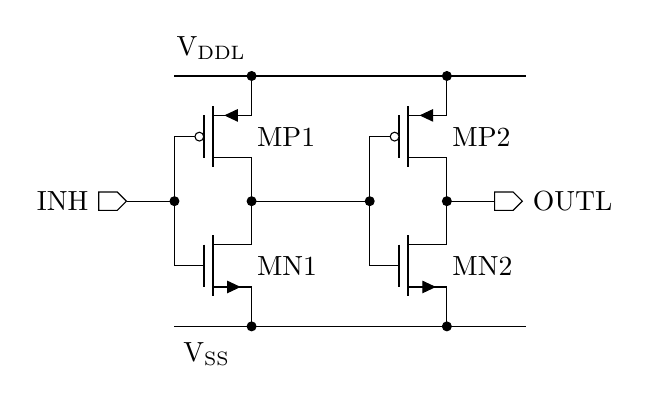
\begin{tikzpicture}[scale=1]
        \ctikzset{tripoles/mos style/arrows}
        \ctikzset{tripoles/pmos style/emptycircle}
        \ctikzset{logic ports=ieee}
        \draw (0,0)
        node[pmos, scale=1](pmos1){MP1}
        (pmos1.D) to [short] ++(0,-0.1) node[nmos, scale=1, anchor=D](nmos1){MN1}
        (pmos1.G) to (nmos1.G)
        ($(pmos1.G)!0.5!(nmos1.G)$) node[circ, scale=1]{} --++ (-0.6,0) node[signal, anchor=east, scale=1, draw](inh){} 
        (inh.west) node[anchor=east, scale=1]{INH}
        ($(pmos1.D)!0.5!(nmos1.D)$) node[circ, scale=1]{} --++(1.5,0) node[circ, scale=1]{}
        (nmos1.center) ++ (1.5,0) node[nmos, scale=1, anchor=G](nmos2){MN2}
        (nmos2.D) to [short] ++(0,0.1) node[pmos, scale=1, anchor=D](pmos2){MP2}
        (nmos2.G) to (pmos2.G)
        ($(pmos2.D)!0.5!(nmos2.D)$) node[circ, scale=1]{} --++ (0.6,0) node[signal, anchor=west, scale=1, draw](outl){}
        (outl.east) node[anchor=west, scale=1]{OUTL}
        (nmos1.G|-nmos1.S) -- (nmos1.S) node[circ, scale=1](vss){} -- (nmos2.S) node[circ, scale=1]{} --++ (1,0)
        (pmos1.G|-pmos1.S) -- (pmos1.S) node[circ, scale=1](vddl){} -- (pmos2.S) node[circ, scale=1]{} --++ (1,0)
	(vss) ++ (-0.15, -0.35) node[left, scale=1]{$\text{V}_\text{SS}$}
	(vddl) ++ (0.05, 0.35) node[left, scale=1]{$\text{V}_\text{DDL}$}
        ;
    \end{tikzpicture}
    \vspace{0.35cm}
    \label{HL_level_shifter}
    }
    \vfil
    \vspace{0.3cm}
    \subfloat[]{
    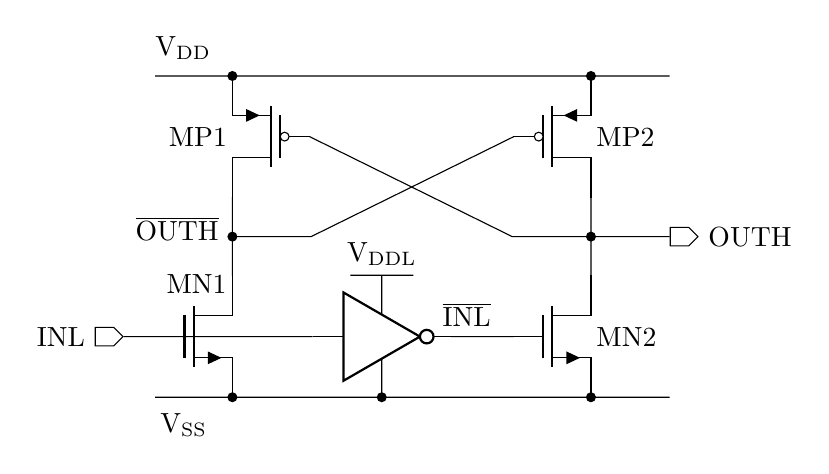
\begin{tikzpicture}[scale=1]
        \ctikzset{tripoles/mos style/arrows}
        \ctikzset{tripoles/pmos style/emptycircle}
        \ctikzset{logic ports=ieee}
        \draw 
        (0,0) node[nmos, anchor=G, scale=1](nmos1){} --++
        (2,0) node[ieeestd not port, anchor=in, scale=1](inv){}
        (nmos1.inner up) ++ (0.05,0.4) node[left, scale=1]{MN1}
        (inv.out) --++ (0.8,0) node[nmos, anchor=G, scale=1](nmos2){MN2} 
        (nmos2.D) --++ (0,0.5) node[circ, scale=1](out){} --++ (0,0.5) node[pmos, anchor=D, scale=1](pmos2){MP2}
        (nmos1.D) --++ (0,0.5) node[circ, scale=1](outb){} --++ (0,0.5) node[pmos, xscale=-1, anchor=D, scale=1](pmos1){\ctikzflipx{MP1}}
        (outb) --++ (1,0) -- (pmos2.G)
        (out) --++ (-1,0) -- (pmos1.G)
        (outb) ++ (-0.05,0.10) node[left, scale=1]{$\overline{\mbox{OUTH}}$}
        (out) --++ (1,0) node[signal, anchor=west, scale=1, draw](out_o){} 
        (out_o.east) node[anchor=west, scale=1]{OUTH}
        (nmos1.G) --++ (-0.4,0) node[signal, anchor=east, scale=1, draw](in){} 
        (in.west) node[anchor=east, scale=1]{INL} 
        (0,0|-nmos1.S) -- (nmos1.S) node[circ, scale=1](vss){} -- (inv.down|-nmos2.S) node[circ, scale=1]{} 
        (inv.down) |- (nmos2.S) node[circ, scale=1]{} --++ (1,0)
        (0,0|-pmos1.S) -- (pmos1.S) node[circ, scale=1](vddh){} -- (pmos2.S) node[circ, scale=1]{} --++ (1,0)
	(vss) ++ (-0.2, -0.35) node[left, scale=1]{$\text{V}_\text{SS}$}
	(vddh) ++ (-0.15, 0.35) node[left, scale=1]{$\text{V}_\text{DD}$}
	(inv.up) --++ (0,0.5) node[above, scale=1](vddl){$\text{V}_\text{DDL}$} ++ (-0.4,0) --++ (0.8,0)
        (inv.out) ++ (0.2,0) node[above, scale=1]{$\overline{\mbox{INL}}$}
        ;
    \end{tikzpicture}
    \label{LH_level_shifter}
    }
    \caption{Шема претварача (а) са високог на низак и (б) са ниског на висок напонски ниво \cite{Osaki:6198744}.}
    \label{Level_shifters}
\end{figure}




\section{Имплементација и резултати симулација} \label{Implementation and results}

\subsection{Симулација рада фреквенцијски затворене петље}

\subsection{PVT зависност дигитално контролисаног осцилатора}

\subsection{Временски прорачун дигитално контролисаног осцилатора}

\subsection{Спектар снаге фреквенцијски затворене петље}

\subsection{Фазни шум дигитално контролисаног осцилатора}


\section{Закључак} \label{Conclusion}


\makebibliography

\end{document}
